\chapter{Desarrollo de prototipos}

\section{Prototipo 1}
\textbf{Objetivo del prototipo}:
Conocer el uso, funcionamiento e implementación de herramientas de cifrado, hashing y generación de CAPTCHAS, con el fin de conocer la integración de estos módulos en diferentes lenguajes de programación.\\
Se implementó un módulo de cifrado de mensajes de texto en lenguaje C++. Tratando de simular el proceso de cifrado del esquema que se esta usando.\\
La primera parte del proceso es abrir el mensaje para lo cual se estan usando los métodos estándar definidos en las bibliotecas nativas de C++, posteriormente se generará una palabra aleatoria de 5 caracteres usando una función Rand()\%100 y transformando el valor de salida a un char.\\
Al resultado se pasa por una función de hashing, esta función no es nativa de ninguna biblioteca estándar de C++ ni de C, por lo que se tuvo que conseguir una en internet y probar que efectivamente funcionara como se necesita.\\
Posteriormente este hash se usará como clave para cifrar el mensaje que ya se ha abierto, para esto se necesita una función AES o DES, ninguna de estas es estándar de alguna biblioteca de C o C++, así que se tendra que buscar y verificar su funcionamiento.\\


\textbf{Conclusión}:
Podemos ver que en C++ el proceso es simple pero se necesita buscar muy bien las bibliotecas externas que se usarán, ya que no siempre están funcionando correctamente, en algunos casos estas ni siquiera compilan.\\
Este caso fue particularmente evidente al buscar una biblioteca de C o C++ que pudiera realizar el cifrado con AES o DES, se encontro con bibliotecas que cifraban mal ya que al meter la misma llave no descifraban e incluso bibliotecas que no se lograron compilar.\\

\section{Prototipo 2}
Se implementó un módulo de cifrado, descifrado y generación de CAPTCHAS en Python, simulando el proceso antes del envío del correo y el que se hace después de la recepción de los correos electrónicos.\\\\\\
Para este se usó el formato estándar del correo electrónico especificado en el RFC 822, también se usaron bibliotecas ya estandarizadas de Python para la implementación de las funciones de hashing, funciones de cifrado y descifrado (AES o DES), funciones aleatorias y la generación de los CAPTCHAS. El codigo fuente de las funciones se encuentra en el Anexo 1.\\

\textbf{Conclusión}:
Se logró generar todo el proceso de envío y parte del proceso de recepción de mensajes. En cuanto al envío se logró leer el mensaje, crear una palabra a partir de funciones random, crear la clave con dicha cadena de caracteres y cifrar el correo exitosamente, además de esto se logró leer el archivo de mensaje de correo electrónico y cifrar únicamente el mensaje que viene en este.\\
Por su parte el módulo de generación de CAPTCHAS mostró muchos problemas para generarlos, ya que no se logró hacer que el intérprete pudiera encontrar correctamente las funciones de la biblioteca de generación CAPTCHAS por lo que al no poder generar un CAPTCHA la recuperación no se puede realizar como se planteó, para verificar únicamente que las funciones trabajan correctamente se implementó el descifrado del mensaje en el mismo método.\\



\section{Prototipo 3}
\textbf{Objetivo}
Generar una imagen un CAPTCHA a partir de una cadena de caracteres ingresada desde una interfaz gráfica.
Este prototipo se construyó en 2 partes; la primera parte fue la interfaz gráfica y sus herramientas, y la segunda en las herramientas para generar la imagen a partir de una cadena de caracteres.\\
Para la interfaz gráfica se utilizaron las siguientes herramientas para desarrollar este prototipo:\\
Biblioteca \textbf{\textit{Qt}} y \textbf{\textit{Qt creator}}: Utilizamos esta biblioteca para generar la interfaz gráfica con la que ingresa la cadena de caracteres y el IDE \textbf{\textit{Qt Creator}} para facilitar la gestión de las clases.\\
La interfaz gráfica consta de un apartado para ingresar la cadena de caracteres y un botón para convertir la cadena a una imagen de CAPTCHAS.\\
Para generar CAPTCHAS se utilizaron las siguientes herramientas:\\
Lenguaje PHP: se utilizó para genera las imágenes CAPTCHAS con la cadena de caracteres proporcionada anteriormente.\\
En un principio se buscó una biblioteca que generara las imágenes CAPTCHAS en el lenguaje C++, pero las bibliotecas de imagenes encontradas no hacen rotaciones, inclinaciones, cambio de tamaños y colores variables para generar CAPTCHAS, por lo tanto las bilbiotecas encontradas tenían que adaptarse a la funcionalidad del prototipo. Por lo tanto se optó por utilizar el lenguaje PHP ya que tiene librerías optimizadas para generar imágenes CAPTCHAS.\\
\textbf{Conclusión.}
La generación de imágenes CAPTCHAS es rápida y fácil de implementar, pero durante la investigación llegamos a la conclusión que el cliente de correo “Thunderbird” está desarrollado en el lenguaje de programación Python y al no tener una biblioteca nativa en el lenguaje C++ para convertir una cadena de caracteres en CAPTCHAS y  se decidió cambiar de lenguaje de programación.\\



\section{Prototipo 4}
\textbf{Objetivo del prototipo.}
Instalar y configurar un servidor de correo electrónico para el envío de mensajes de correo electrónico entre diferentes usuarios.\\
Instalación y configuración de un servidor de correo electrónico y un servidor DNS.\\


Para el desarrollo de este prototipo fue necesario instalar el servidor de correo electrónico con el protocolo pop y imap, un cliente de correo electrónico web, un servidor DNS y el servidor HTTP Apache. Estos 3 servicios se levantaron en una computadora con un sistema operativo Xubuntu 15.04; primero se instaló el servidor HTTP\cite{HTTP}, posteriormente se pasó a la instalación del servidor DNS y configuración de un dominio\cite{DNS}; se seguió con la instalación del servidor de correo electrónico y los protocolos pop y imap; y por último se instaló y  configuró el cliente de correo web\cite{web}.\\
Para la instalación de servidor HTTP fue necesario seguir los siguientes pasos:\
\begin{itemize}
 \item Se abre una terminal en Ubuntu y se escribe el comando: “sudo apt-get install apache2”
 \item Se abre como administrador el archivo /etc/apache2/sites-enabled/00-default.conf y se escribe la siguiente configuración:
 \begin{lstlisting}[frame=single]
  <VirtualHost *:80>
     ServerAdmin nombredelsitio@example.com
     ServerName nombredelsitio
     ServerAlias www.nombredelsitio.com
     DocumentRoot /var/www/nombredelsitio.com/public_html/
     ErrorLog /var/www/nombredelsitio.com/logs/error.log
     CustomLog /var/www/nombredelsitio.com/logs/access.log
      combined
</VirtualHost>
 \end{lstlisting}
 \item Se levanta el servicio http con el siguiente comando: “sudo service apahce2 start”
 \item Para verificar la instalación Se abre un explorador y escribirlos en la barra de búsqueda la siguiente dirección: http://localhost/ y nos aparecerá la siguiente pantalla.
\end{itemize}


Una vez instalado el servidor HTTP se prosigue a instalar el servidor DNS, para levantar este servicio es necesario seguir los siguientes pasos:
\begin{itemize}
 \item Se selecciona un nombre de dominio, para fines prácticos nuestro dominio privado será “correocifrado.edu”.
 \item Se abre una terminal en Ubuntu y se escribe el siguiente comando: “sudo apt-get install bind9”
 \item Realizar una copia de respaldo del archivo de configuración original con el comando “cp /etc/bind/named.conf.local \\ /etc/bind/named.conf.local.original”
 \item Se edita el archivo de configuración con: “nano /etc/bind/named.conf.local”
 \item Se agrega al final del archivo lo siguiente:
 \begin{lstlisting}[frame=single]
  zone "correocifrado.edu" {
  type master;
  file "correocifrado.edu.zone";
  };

  zone "10.168.192.in-addr.arpa" {
  type master;
  file "db.192.168.10";
  };
 \end{lstlisting}
 \item Se procede a crear los (nuevos) archivos de zona, esos archivos contienen los registros del DNS y en Ubuntu se encuentran en el directorio /var/cache/bind/ “nano /var/cache/bind/db.isti.edu.ni.zone”
 \item En el archivo Se agrega el siguiente texto:
 \begin{lstlisting}[frame=single]
  $ORIGIN correocifrado.edu.
$TTL 86400            ; 1 dia
@  IN  SOA ns.correocifrado.edu. info.correocifrado.edu. (
        2014112401    ; serie
        6H            ; refresco (6 horas)
        1H            ; reintentos (1 hora)
        2W            ; expira (2 semanas)
        3H            ; minimo (3 horas)
)

@      IN       NS     ns
@      IN       MX 10  mail
ns     IN       A      192.168.10.10
mail   IN       A      192.168.10.10
www    IN       A      192.168.10.10
 \end{lstlisting}
 \item De igual manera el archivo de zona de búsqueda inversa:\\
  nano /var/cache/bind/db.192.168.10
  \item Se agrega la siguiente configuración:    
  \begin{lstlisting}[frame=single]
   $ORIGIN 10.168.192.in-addr.arpa.
$TTL 86400     ; 1 dia
@  IN  SOA ns.correocifrado.edu. info.correocifrado.edu. (
        2014112401    ; serie
        6H            ; refresco (6 horas)
        1H            ; reintentos (1 hora)
        2W            ; expira (2 semanas)
        3H            ; minimo (3 horas)
)
\end{lstlisting}
\begin{lstlisting}[frame=single]
@       IN      NS     correocifrado.edu.
10      IN      PTR     correocifrado.edu.
10      IN      PTR     mail.correocifrado.edu.
10      IN      PTR     www.correocifrado.edu.
  \end{lstlisting}
  \item Se procede a re-iniciar el servicio con el comando “service bind9 restart”
  \item Cambiar el primero de los servidores DNS por la IP del nuestro: “nameserver 192.168.10.10”
  \item Por último se ejecuta el siguiente comando “nslookup www.correocifrado.edu” y nos dará un resumen de los DNS configurados.
\end{itemize}
Se prosigue con la instalación del servidor de correo electrónico y los servicios del protocolo pop y imap con la aplicación courier-pop y courier-imap:
\begin{itemize}
 \item Se abre una terminal y se escribe el siguiente comando: “sudo apt-get install postfix”
 \item Durante la instalación aparecerá una pantalla de configuración, se da enter para aceptar la configuración.
 \item En tipo genérico de configuración de correo se selecciona "Sitio de Internet".
 \item A continuación se indica el nombre de sistema de correo, normalmente la dirección del dominio registrado, en este caso "cifradocorreo.net".
 \item Con esto se verá que postfix termina de instalarse y se procede a editar el archivo “/etc/postfix/main.cf”.
 \item Se añade al final del fichero main.cf las líneas:
 \begin{lstlisting}[frame=single]
  inet_protocols = ipv4
home_mailbox = emails/
 \end{lstlisting}
 \item Una vez guardado el archivo que se edita se procede a reiniciar el servidor con el comando “sudo /etc/init.d/posrfix restart”
\end{itemize}


Una vez instalado el servicio de correo electrónico se procede a instalar el courier-pop y el courier-imap.
\begin{itemize}
 \item Se abre una terminal el Ubuntu y se escribe el siguiente comando “sudo apt-get install courier-pop”.
 \item Nos mostrará una ventana de configuración de courier-base, se selecciona “NO”.
 \item Se procede a instalar courier-imap con el siguiente comando “sudo apt-get install courier-imap”.
 \item Se espera a que finalice la instalación.
\end{itemize}


Por último es necesario instalar una aplicación webmail para enviar correos entre usuarios del correo electrónico.
\begin{itemize}
 \item Se abre una terminal en Ubuntu y se escribe el siguiente comando “sudo apt-get install squirrelmail”.
 \item Tras la instalación de SquirrelMail se configura ejecutando el siguiente comando “sudo squirrelmail-configure”
 \item Se selecciona la letra D y se da enter.
 \item En este nuevo menú se teclea la opción courier y se da enter.
 \item Nos dará un informe de la configuración que se selecciono y se da enter para continuar.
 \item Se regresa al primer menú, ahora se teclea el número 2 y se da enter.
 \item Se selecciona en este nuevo menú la opción 1 y se da enter nuevamente.
 \item Pedirá nuestro nombre de dominio, en este caso es el dominio que se configuró en el servidor DNS “correocifrado.net”
 \item Regresará al menú principal y se teclea la letra Q para salir de la configuración.
 \item Preguntará si queremos guardar los cambios y se teclea la letra Y.
 \item Por último se ejecuta el siguiente comando para levantar SquirrelMail en Apache “sudo ln -s /usr/share/squirrelmail /var/www/webmail”
 \item Se reinicia el servicio apache con el comando “sudo service restart apache2”.
 \item Se podra entrar a la aplicación escribiendo el explorador “www.correocifrado.edu/webmail”
\end{itemize}


Para poder enviar correos se necesitan usuarios que desean enviar mensajes entre usuarios, primero se creará un usuario
\begin{itemize}
 \item Se abre una terminal de Ubuntu y se escribe el siguiente comando “sudo adduser nombreusuario”.
 \item Se introduce la nueva contraseña de UNIX: introduciremos la contraseña para el usuario, es importante que sea segura (números, letras, mayúsculas y minúsculas) pues con el usuario y la contraseña podremos acceder vía web al servidor de correo electrónico desde cualquier parte del mundo.
 \item Vuelva a escribir la nueva contraseña de UNIX: se repite la contraseña.
 \item Full Name: Se introduce el nombre completo, por ejemplo ``Alicia Robles Maldonado''.
 \item Room Number: Número de oficina.
 \item Work Phone: teléfono del trabajo.
 \item Home Phone: teléfono particular.
 \item Other: otros datos del usuario.
 \item Se responde ``S'' a la pregunta ``¿Es correcta la información?''. Y se tendrá el usuario creado en el sistema operativo, que también servirá como usuario (buzón) para el servidor de mail.
 \item Ahora se generará el buzón con el siguiente comando “sudo maildirmake /home/nombreusuario/emails”
 \item Se cambian los permisos de las carpeta emails con el comando “sudo chdown nombreusuario:nombreusuario /home/nombreusuario/emails -R
\end{itemize}
Para crear otro usuario es necesario repetir los pasos anteriores.
\section{Prototipo 5}
\textbf{Objetivo:} Familiarizarse con el uso de la tecnología y estructura del cliente de correo electrónico Thunderbird.\\
Se planeó la creación de un completo para el cliente de correo electrónico Thunderbird, para dar paso al desarrollo del complemento es necesaria la documentación de dicho cliente de correo, la cual debe de ser debidamente requisitada a su desarrollador que en este caso es Mozilla. 
El cliente Thunderbir al ser un cliente de software libre debe de contar con una documentación pública. Al buscar documentación en la página de desarrollo de Mozilla resulta evidente que no está, pero puede ser pedida a Mozilla por medio de la misma página. La documentación fue pedida el 03-03-16 y a la fecha de escritura de este reporte 20-04-16 no se ha obtenido una respuesta por parte de Mozilla.\\
\textbf{Conclusión:} Por el tiempo de respuesta y la falta de documentación implementar un complemento para thunderbird en el tiempo proporcionado para este trabajo terminal no es viable.
\section{Prototipo 6}
\textbf{Objetivo:} Familiarizarse con el uso de las tecnologías y estructuras de Nylas N1, así como verificar su viabilidad como solución factible para el presente trabajo.\\
La documentación de este cliente de correo electrónico es fácil de conseguir ya que es pública directamente en su página oficial, además de contar con breves tutoral de como usarse.
Se implementó sobre la interfaz incluir imágenes y mostrar información nueva sobre el panel auxiliar, también la obtención directa del cuerpo del mensaje para poder procesarlo, agregar una clase dentro del complemento que permita la comunicación con el servidor de CAPTCHAS.

\begin{itemize}
 \item Inclusión de texto e imagen en la interfase: El mismo N1 da la posibilidad de generar tu propio complemento de correo ya que el mismo te proporciona un formato estándar y una opción para modificar los textos de sus diferentes áreas, se modifico justo la opción de texto en la barra lateral derecha pero para agregar una imagen y texto al mismo tiempo.
 \item Obtención del cuerpo del mensaje: Despues de analizar la estructura del complemento se creo uno propio en el cual se mandaron llamar el cuerpo del mensaje y el asunto por medio de métodos que el mismo N1 proporciona.
 \item Comunicación con el servidor de CAPTCHAS: En complemento creado por nosostros se generó una clase que hace una llamada al servidor de CAPTCHAS que espera una respuesta para poder empaquetar el nuevo cuerpo del mensaje y poder mandarlo por correo. Todas estas clases están implementadas en CoffeScript este lenguaje no es secuencial si no concurrente, como la función de empaquetamiento del cuerpo espera la respuesta del servidor y esta no llega si no hasta después de que ya se ejecutó esta función genera un error.
\end{itemize}
\textbf{Conclusión:} No es posible hacer una sincronización con los servidores externos que necesitamos, por lo que la implementación no es viable en Nylas N1.

\section{Prototipo 7}
\textbf{Objetivo:} Evaluar la viabilidad y compatibilidad del algoritmo de cifrado así como su integración con Nylas N1.\\
Se implementaron los algoritmos de cifrado, descifrado, generación de llave y generación de CAPTCHA en el lenguaje JavaScript. considerando que Nylas N1 esta implementado en CoffeScript que es una versión de escritorio de JavaScript.
\begin{itemize}
 \item Generación de llave: Se genera una cadena de caracteres aleatorio de tamaño 5. Primero se genera un número aleatorio del 0 al 63 y este se manda a otra función que lo mapea a su caracter correspondiente en el anillos $AL=\{A-Z\}\cup \{a-z\}\cup \{0-9\}\cup \{+,/\}$ 
 \begin{lstlisting}[frame=single]
  var map;map = [];
  
map=["A","B","C","D","E","F","G","H","I","J","K","L","M","N"
,"O","P","Q","R","S","T","U","V","W","X","Y","Z","a","b","c"
,"d","e","f","g","h","i","j","k","l","m","n","o","p","q","r"
,"s","t","u","v","w","x","y","z","0","1","2","3","4","5","6"
,"7","8","9","+","/"];
//alert(map.length);

function CtoI(let){
	var a;
	for (var i = 0; i < map.length; i++) {
		if (map[i]==let) {
			a=i;
			//alert(a);
		}
	}
	return a;
}

function ItoC(num){
	return map[num];
}
 \end{lstlisting}
 de esta cadena generaremos un digesto por medio de una función hash sha256 y recortada a una cadena de caracteres tamaño 16 la cual se usará como llave para la función de cifrado.
\item Cifrado: se cifra el texto con una función AES 128bits usando la llave generada anteriormente
\item Generación de CAPTCHA: JavaScript no tiene metodos propios de edición de imagen ni bibliotecas de creación de CAPTCHAS, pero se pueden pasar las variables declaradas en JavaScript a PHP y que este lenguaje termine el proceso, solo que es necesaria la creación de un formulario HTML para que esto suceda, en el caso nuestro esto no es factible ya que Nylas N1 no hace uso de estas herramientas.
\end{itemize}
\begin{lstlisting}[frame=single]
 var semilla="";
for (var i = 0; i < 5; i++) {
	var r = Math.floor((Math.random() * 63) + 1);
	semilla=semilla + ItoC(r);
}

alert(semilla);

var shaObj = new jsSHA("SHA-1", "TEXT");
shaObj.update(semilla);
var hash = shaObj.getHash("HEX");

alert(hash);
var llave;
llave = hash[0];
//llave = llave + hash[1];
for (var i = 1; i < 16; i++) {
	llave=llave + String(hash[i]);
}
alert(String(llave));

usedKey=llave;
myStr="Osama Oransa2012Osama Oransa2011RashaOsama Oransa2012Osa  
Oransa2011RashaOsama Oransa2012Osama Oransa2011RashaOsama 
Oransa2012Osama Oransa2011Rasha";
alert(myStr);

var key=init(usedKey);
alert(key);
encrypted=encryptLongString(myStr,key);
alert('after encrypt='+encrypted);
decrypted=decryptLongString(encrypted,key);
alert('after decrypt='+decrypted);
finish();

\end{lstlisting}
\textbf{Conclusión:} El uso de JavaScript para implementar el esquema propuesto en este trabajo no es totalmente posible ya que el mismo lenguaje no nos permite la creación de CAPTCHAS ni la llamada a sistema por lo que limita la capacidad de desarrollo.

\section{Prototipo 8}
\textbf{Objetivo:} Crear una biblioteca en lenguaje Python que contenga el esquema de cifrado por CAPTCHA.
El cliente de correo electrónico Thunderbir tiene una parte implementada en python, pensado para esto se implemento el presente esquema en el lenguaje Python. Para continuar con el desarrollo del presente trabajo se decidió crear una biblioteca en el lenguaje Python.\\
En esta biblioteca se implementaron en métodos por separado: la creación de la cadena original llamada semilla, la creación de la llave, la creación del CAPTCHA, cifrado y descifrado.
En esta biblioteca se esta considerando un esquema en el cual se pueda generar un solo CAPTCHA por mensaje cifrado o "n" número de CAPTCHA's por cada mensaje cifrado, para el esquema multi CAPTCHA se hace uso de el algoritmo de secreto compartido por lo que para este se implementaron los metodos: Codificación, decodificación, repartir el secreto y recuperar el secreto. El código fuente se encuentra en el Anexo 2.
\begin{itemize}
 \item Crear Semilla: para este método originalmente esta configurado para hacer una palabra de 5 caracteres, pero puede introducir manualmente el numero de caracteres deseados, esto es generando 5 números aleatorios en un rango de 0 a 63 que posteriormente son asignados a su correspondiente caracter en el anillo $AL=\{A-Z\}\cup \{a-z\}\cup \{0-9\}\cup \{+,/\}$ 

 \item Crear Llave: En este método se manda la semilla y a esta se le genera un digesto con una función SHA256 	que posteriormente es recortada a 16 bits.

 \item Crear CAPTCHA: este método recibe la opción, la semilla, y el asunto. La opción define cual es el funcionamiento de este método, si la opción es 0 el método toma la semilla y crea un CAPTCHA a partir de ella usando la biblioteca CAPTCHA de Python. Por el contrario si la opción es 1 lo que recibe la función en el parametro semilla, es un arreglo de caracteres y uno a uno lo convierte en CAPTCHA.
En el caso particular de la generación de CAPTCHAS, se modificó la biblioteca que los crea, ya que esta función arrojaba CAPTCHAS ilegibles.

\item Codificar: La función Codificar toma como parámetro, una cadena de caracteres y la transforma en un número entero, primero caracter a caracter se busca su correspondiente número entero en el anillo $AL$ posteriormente este se pasa a una representación en 6 bits y por último se convierte a un número entero.

\item Decodificar: La función decodificar recibe como parámetro un número entero y el número de partes en las que tiene que partir el número, esto lo hace convirtiendo el número entero a su representación binaria, posteriormente se separa en números binarios de 6 bits y cada uno es convertido en un número entero e intercambiado por su correspondiente caracter del anillo $AL$.

\item Generar Partes: Se reciben como parámetro el anillo $Zp$ , el número de partes en que se dividirá el secreto $w$, el número de partes necesarias para recuperar el secreto $t$ y el secreto $k$. Se generan aleatoriamente $w$ que son las $x$ e igualmente de manera aleatoria se generan $t$ elementos que son los elementos $a$, con esto se genera la sumatoria correspondiente para generar los elementos $y$. La función retorna pares de números que están conformados por $x,y$.

\item Recuperar secreto: por medio del algoritmo de Lagrange se resuelve el sistema de ecuaciones y así recuperando el secreto

\item Cifrar: Este método recibe como parámetro el cuerpo del mensaje, el asunto y de manera opcional recibe la opción de cifrado, el número de caracteres de los CAPTCHAS, el número de partes en que se divide el secreto, y el número de pares necesarios para recuperar el secreto.
Este método hace las funciones de un main, ya que en este método se invocan todos los demás para poder realizar el funcionamiento del esquema completo. Este método tiene dos funciones, la primera es la opción 0 en la que se crea la semilla, se calcula el anillo $Zp$, con la semilla se crea el CAPTCHA con opción 0, con la semilla se crea la llave y con esta se procede a cifrar el cuerpo del mensaje siempre cuidando que los bloques sean del tamaño de la llave, en este caso el meto retorna el cuerpo cifrado y la ruta en la que están los CAPTCHAS.
Este método en opción 1 genera la semilla, despues calcula $Zp$, mapea a número la semilla por medio de Codificar, con este número se generan los pares del secreto compartido, estos son mapeados a cadena de caracteres y convertidos en CAPTCHAS, se crea la llave y por último se cifra el cuerpo del mensaje con esta, en este caso el método retorna el cuerpo del mensaje cifrado y una lista de pares donde esta el número x y su correspondiente imagen CAPTCHA.

\item Descifrar: este método hace le proceso inverso que el método cifrar, este recibe como parámetro el cuerpo cifrado, una cadena con el CAPTCHA o una lista de pares, $x,CAPTCHA$.
Con la opción 0 recibe una cadena de caracteres en la opción CAPTCHA con este se genera la llave y se descifra el cuerpo obteniendo el mensaje original. En caso de tener la opción 1 se recibe en el parámetro CAPTCHA una lista que contiene los pares $x,CAPTCHA$
 de este se obtiene el tamaño del CAPTCHA y se calcula el anillo $Zp$, con esto se toman los CAPTCHAS y se mapean a su representación numérica por medio de Codificar, los pares de números se ingresan al método que calcula el secreto compartido, lo arrojado por este método se
 mapea a su representación en cadena de caracteres y se genera la llave con esto se descifra el cuerpo del mensaje y se obtiene el mensaje original. Este metodo retorna el cuerpo del mensaje original.

\end{itemize}
\textbf{Conclusión:} La funcionalidad de la biblioteca ya implementada, corresponde al esquema propuesto en “On Securing  Communication  from Profilers”, al tener todas las funciones separadas lo hace tener una funcionalidad modular. Esta implementación se usará para integrarla al siguiente prototipo.
\pagebreak
\section{Prototipo 9}
\textbf{Objetivo:} Dar de alta un servidor en el lenguaje PHP donde se alojen, busquen y se realice el intercambio de CAPTCHAS entre los usuarios que utilicen los protocolos P y P’ del esquema Díaz – Chakravorti.

En éste prototipo se tienen implementados por separado 3 archivos PHP que se encargan, cada uno, de dan de alta a los usuarios que desean utilizan el esquema “On Securing  Communication  from Profilers”; subir al servidor los CAPTCHAS que contiene la clave de descifrado de los mensajes redactados por los usuarios previamente registrados; y realizan la descarga de los mismos al momento de que el usuario destino desee recuperar el mensaje, esto con el fin de poder hacer el intercambio y resguardo de las claves para el descifrado de los mensajes de correo electrónico entre usuarios registrados. Tambien se cuenta con una base de datos que nos guarda la relación entre los mensajes enviados y los CAPTCHAS que contienen la clave para ser descifrados. El código fuente de encuentra en el anexo 3
\begin{itemize}
 \item Alta de usuarios: El servidor cuenta con un archivo PHP donde recibe las peticiones de los nuevos usuarios que quieran hacer uso de los protocolos P y P’ bajo el esquema propuesto en este documento, este archivo PHP recibe un formulario HTML llenado previamente con el correo electrónico del usuario, nombre de usuario que lo identificara en el servidor y una contraseña. El nombre de usuarios y la contraseña son utilizados para autenticar a los usuarios y se lleve un control de los CAPTCHAS que se tienen listos para ser intercambiados. \\
 La respuesta entregada por este archivo PHP es una respuesta HTML, la cual contiene la respuesta con codigos para saber si se realizo correctamente la operacion.

 \item Cargar CAPTCHAS: Este servidor cuenta con un archivo PHP que recibe las peticiones de los usuarios ya registrados que quieren subir los CAPTCHAS generados por los protocolos P y P’. La carga de los CAPTCHAS se hace mediante un formulario HTML llenado previamente y archivo PHP se encarga de darnos un código para saber si la carga de los CAPTCHAS fue realizada satisfactoriamente.

 \item Descargar CAPTCHAS: Por último, el servidor cuenta con un archivo PHP que recibe por medio de un formulario HTML el correo destino, el correo origen y la firma que identifica al mensaje de correo electrónico que se desea descifrar. Este archivo nos devuelve una URL para descargar los CAPTCHAS deseados ó un mensaje de error en caso de pedir los CAPTCHAS de un mensaje inexistente en la base de datos.

\end{itemize}
\textbf{Conclusión:} La funcionalidad de este servidor es simple ya que se limitan a la distribución y resguardo de los CAPTCHAS generados por los usuarios registrados que utilizan los protocolos P y P’ del prototipo anterior. Su implementación corresponde al esquema propuesto en “On Securing  Communication  from Profilers” y se integra en el prototipo siguiente para completar dicho esquema.
\pagebreak
\section{Prototipo 10}

\textbf{Objetivo:} Crear un cliente de correo electrónico de escritorio que utilice el esquema descrito en este documento.

El cliente de correo electrónico se programó utilizando la biblioteca grafica GTK3+, el entorno gráfico de GNOME 3 y el lenguaje de programación Python. Para poder inicial el desarrollo de este prototipo es necesario instalar previamente la biblioteca gráfica GTK3+ y el entorno gráfico GNOME 3, ver anexo 4. 

Se inicio el desarrollo de este prototipo generando una interfaz gráfica que ayude a establecer las configuraciones básicas para conectarse con los servidores de correo electrónico por los protocolos POP3 y SMTP. Esta interfaz también establece la configuración necesaria para conectarse con el servidor de CAPTCHAS y para escoger el protocolo de cifrado de mensajes que se utilizará.
\begin{itemize}
 \item Configuración básica POP3: El cliente de correo electrónico establece una conexión POP3 con un servidor de correo electrónico para poder descargar los mensajes de un usuario, para poder hacerlo se necesita nombre de host, puerto de comunicación, nombre de usuario, contraseña del usuario y si se utilizara una conexión segura. Todos estos datos son proporcionados por el servidor de correo electrónico con el que se desea comunicar.
 \item Configuración básica SMTP: El envío de mensajes de correo electrónico se realiza estableciendo una comunicación con nuestro servidor de correo electrónico, para ello se necesita nombre de host, puerto de comunicación, nombre de usuario y contraseña del usuario. Al igual que en la configuración POP3 estos datos son proporcionados por el servidor de correo electrónico con el que se desea comunicar.
 \item Configuración con el servidor de CAPTCHAS: El envío de la imágenes CAPTCHAS generadas después del cifrado de los mensajes necesitan ser resguardadas en el servidor de CAPTCHAS, prototipo 9, para ello es necesario enviar al servidor su dirección de correo electrónico, un nombre de usuario y una contraseña. El servidor valida si el usuario ya esta registrado, en caso contrario el servidor realiza el registro del usuario con los datos proporcionados.
\end{itemize}
Estas 3 configuraciones se establecen llenando los campos de la interfaz, ver figura n, la cual llamaremos ventana de configuración. Esta ventana genera un archivo JSON donde se guardan estos datos para poder ser utilizado mas adelante para el envío y recepción de mensajes de correo electrónico, así como la subida y descarga de las imágenes CAPTCHA y la selección entre los protocolos P y P’ para cifrar los mensajes de correo electrónico.

\begin{figure}[H]
\centering
	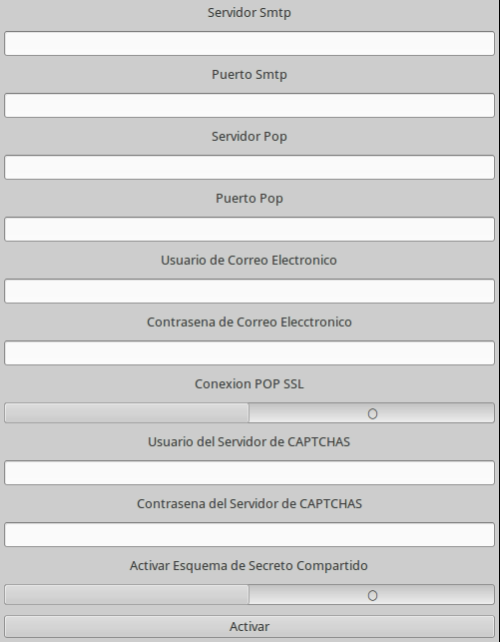
\includegraphics[width=10cm, height=10cm]{./images/VentanaConfig.png}
	\caption{Ventana de Configuración}
	\label{fig:6-10-1}
\end{figure}

Posteriormente se genero una interfaz gráfica principal para visualizar los mensajes de correos electrónicos y una segunda interfaz para la redacción de los mismos.

\begin{figure}[H]
\centering
	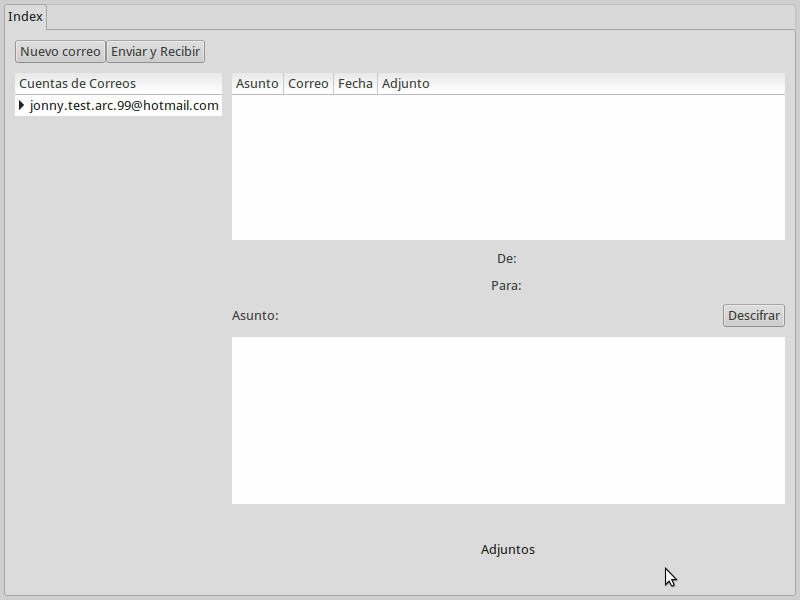
\includegraphics[width=15cm, height=10cm]{./images/VentanaPrincipal.png}
	\caption{Ventana Principal}
	\label{fig:6-10-2}
\end{figure}

La primera  interfaz, tambien llamada ventana principal, esta dividida en 3 parte una barra lateral, un listado y un visualizador de mensajes de correo electrónico. En la barra lateral encontramos las carpetas donde se almacenan los correo electrónicos, en el listado encontramos los mensajes de correos electrónicos que se han almacenado en la carpeta seleccionada de la barra lateral y por ultimo tenemos el visualizador de mensajes, el cual  despliega la dirección de correo del usuario que mando ese mensaje, los destinatarios a donde fue dirigido el mensaje y por ultimo el cuerpo del mensaje, ver figura n.

La segunda interfaz, también llamada ventana de envío de mensajes,  tiene un diseño simple para redactar los mensajes de correo electrónico, esta interfaz cuenta con 3 espacios, el primero es para escribir la dirección de correo donde se enviará el mensaje; el segundo espacio es para escribir el asunto que se adjunta al mensaje; y por último espacio es para la redacción del mismo, ver figura n.
\begin{figure}[H]
\centering
	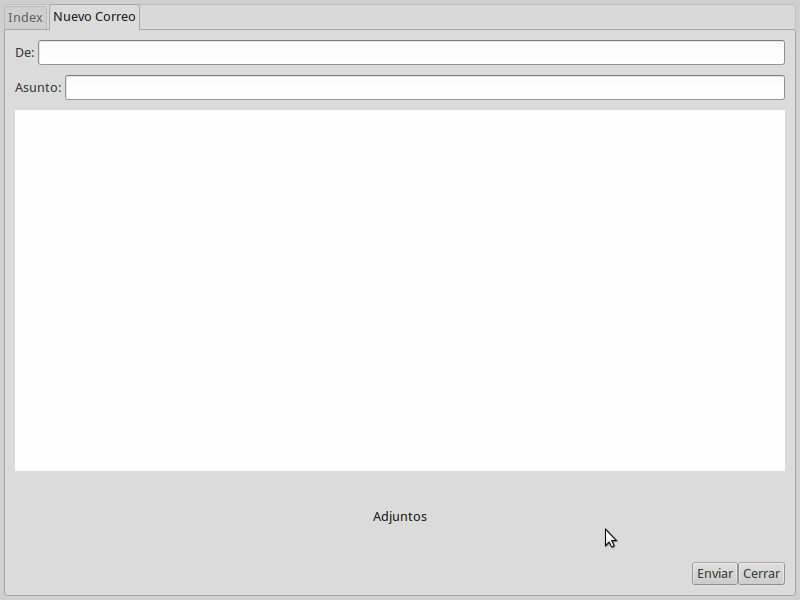
\includegraphics[width=15cm, height=10cm]{./images/VentanaNewCorreo.png}
	\caption{Ventana de Nuevo Correo}
	\label{fig:6-10-3}
\end{figure}
Una vez que se tienen las interfaces listas se procede a darles funcionalidad, para ello se llevan a cavo las siguientes actividades.
\begin{itemize}
 \item Cifrado de mensajes de correo electrónico por el protocolo P y P’: Esta actividad se inicia al redactar un correo electrónico en la ventana de envío de mensaje y pulsar el botón enviar. 
Lo primero que hace es toma la fecha actual de la computadora y la concatena con las dirección de correo destino y origen, a esta cadena generada  se le  obtiene un digesto MD5, el cual sera utilizado como firma para el mensaje de correo. Posteriormente se toma el mensaje redactado por el usuario y es enviado a la biblioteca de cifrado, prototipo 8, especificando el protocolo a usar. Esta biblioteca nos regresa el mensaje cifrado junto con la ruta de la imágenes CAPTCHAS que descifran el mensaje, Después se toma este mensaje cifrado y es concatenado con la firma generada anteriormente  y con una cabecera que nos indicara si el mensaje esta cifrado o no al momento de visualizarlo. Por ultimo se toman las direcciones de correo, origen y destino, el asunto redactado y el mensaje cifrado para generar un mensaje de correo electrónico y guardalo en la carpeta de salida, éste mensaje será enviado posteriormente por el protocolo SMTP al servidor de correos. Por ultimo esta actividad activa el envío de imágenes CAPTCHAS al servidor de CAPTCHAS.
 
 \item Envío de imágenes CAPTCHAS al servidor de CAPTCHAS: Esta actividad se inicia al momento de pulsar el botón “Enviar y Recibir” de la ventana principal o al termino del cifrado de mensajes de correo electrónico.
Esta actividad inicia tomando un listado de los mensajes de correo que se tienen pendientes de envío en la carpeta de salida y buscando los CAPTCHAS correspondientes a cada mensaje. Cada uno de estos CAPTCHAS son enviados al servidor junto con las direcciones de correo origen y destino, la firma del mensaje de correo y los datos de configuración del archivo JSON por medio de una petición HTTP. Por último, por cada CAPTCHA enviado exitosamente se envía su correspondiente mensaje al servidor de correo por el protocolo SMTP.
 \item Envío de mensajes por el protocolo SMTP: Esta actividad se inicia al momento de pulsar el botón “Enviar y Recibir” de la ventana principal o al termino de un envío exitoso de un CAPTCHA.
Para hacer el envío de un mensaje de correo electrónico se necesitan los datos de configuración que se tienen el el archivo JSON junto con el mensaje que se desea enviar. En caso de error el mensaje se almacena en la carpeta de salida.
 \item Descargar mensajes por POP3: Esta actividad se inicia al momento de pulsar el botón “Enviar y Recibir” de la ventana principal.
Para iniciar la descarga de los mensajes de correo electrónico se toman los datos básicos del archivo JSON para establecer comunicación con el servidor. Una vez establecida la conexión el servidor de correo electrónico nos dará uno a uno los mensajes y el cliente de correo electrónico guardará cada mensaje en un archivo txt en la carpeta de entrada.
 \item Descarga de imágenes CAPTCHAS del servidor de CAPTCHAS: Esta actividad se inicia al momento de pulsar el botón “Descifrar” de la ventana principal.
Para saber si el mensaje esta cifrado se busca en el cuerpo del mensaje la cabecera de cifrado de donde obtenemos la firma del mensaje. Con la firma del mensaje se buscan las imágenes de descifrado en la carpeta CAPTCHA, esta carpeta se crea con la instalación del prototipo, en caso de no encontrar las imágenes en la carpeta el cliente de correo hacer una petición HTTP al servidor de CAPTCHAS adjuntando la firma del mensaje, las direcciones de origen y la dirección destino.
El servidor contesta enviando la dirección URL de la imágenes de  donde  el cliente descarga las imágenes y las guarda en la carpeta CAPTCHA. Después de guardarlas, el cliente despliega la o las imágenes CAPTCHA en una ventana para que el usuario lo resuelva, esta ventana la llamaremos ventana de Descifrado. El despliegue de una o mas imágenes dependerá del protocolo que se haya utilizado para cifrar.
\begin{figure}[H]
\centering
	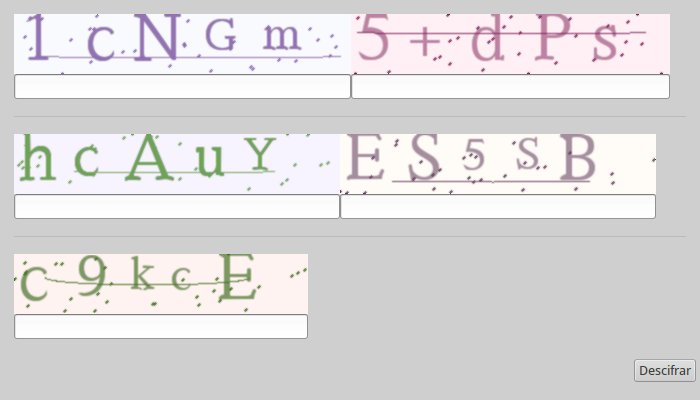
\includegraphics[width=15cm, height=7cm]{./images/VentanaMultiCAPTCHAS.png}
	\caption{Ventana Multi-CAPTCHAS}
	\label{fig:6-10-4}
\end{figure}
 \item Descifrado de mensajes de correo electrónico por el protocolo P y P’: Esta actividad se inicia al momento de pulsar el botón “Descifrar” de la ventana de Descifrado.
Una vez que el usuario resuelve los CAPTCHAS se toman las respuestas junto con el cuerpo del mensaje cifrado sin la cabecera de cifrado y se envían a la biblioteca de cifrado, prototipo 8, la cual nos regresa el texto descifrado. En caso de que los CAPTCHAS sean ingresados incorrectamente el texto regresado por la biblioteca sera ilegible y el cliente de correos lo detectara.

\begin{figure}[H]
\centering
	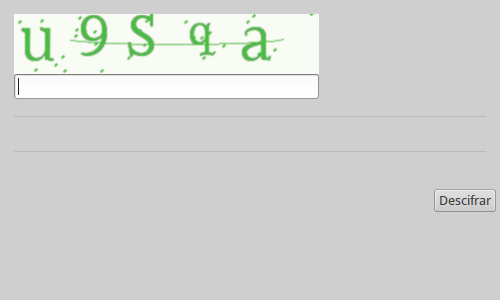
\includegraphics[width=10cm, height=5cm]{./images/VentanaCAPTCHA.png}
	\caption{Ventana CAPTCHAS}
	\label{fig:6-10-5}
\end{figure}

\end{itemize}
\textbf{Conclusión:}  El cliente de correo electrónico que se describió en este prototipo es completamente funcional y en conjunto con los prototipos 8 y 9 cumplen con el funcionamiento del esquema propuesto en este documento para implementar los protocolos P y P’ del esquema Díaz -Chakravorti. Para ver el codigo completo del prototipo 10 ver el anexo 5.